\begin{comment}
	\pagebreak
\end{comment}

\section{Parametric Body Models}

\textbf{LBS:} $t'_i = \sum_k w_{ki} G_k(\theta, J) t_i$\\
\begin{comment}
	$t, t'$ Rest/ Transformed vertices\\
	$w_{ki}$: Blend skinning weights (given by designer)\\
	$G_k$: Rigid bone transformation\\
	$\theta$: Pose\\
	$J$: Joint locations\\
	
	\begin{Figure}
 		\centering
 		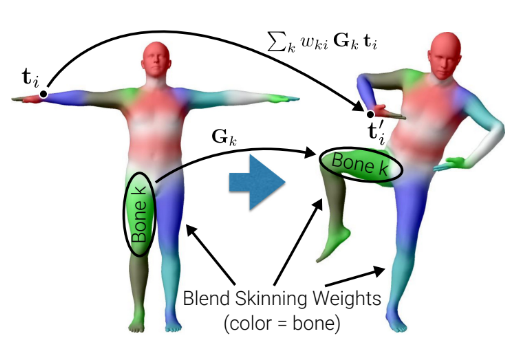
\includegraphics[width=\linewidth]{graphic/pbm-lbs}
 		\captionof{figure}{PBM Linear Blend Skinning}
	\end{Figure}
\end{comment}

\textbf{SMPL:} $t'_i = \sum_k w_{ki} G_k(\theta, J(\beta)) (t_i + s_i(\beta) + p_i(\theta))$\\
\begin{comment}
	Differences to the standeart Linear Bend Skinning is that
	\begin{itemize}
	\item Joints J depend on shape beta
	\item Shape correctives s
	\item Pose correctives p	
	\end{itemize}
\end{comment}

\textbf{Pipeline:} Template mesh, joint locations, shape to body shape, add pose correction, LBS\\

\textbf{Learned GD:} $\Theta^{t+1} = \Theta^t + F(\frac{\partial L}{\partial \Theta}, \Theta^t, x)$\\
\begin{comment}
	\begin{Figure}
 		\centering
 		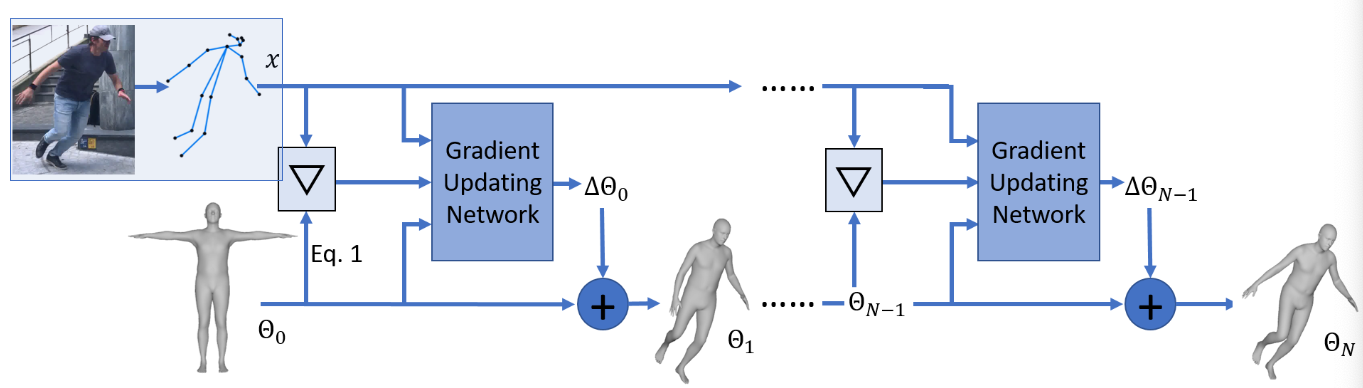
\includegraphics[width=\linewidth]{graphic/pbm-inference}
 		\captionof{figure}{PBM Inference Pipeline}
	\end{Figure}
	
	\begin{Figure}
 		\centering
 		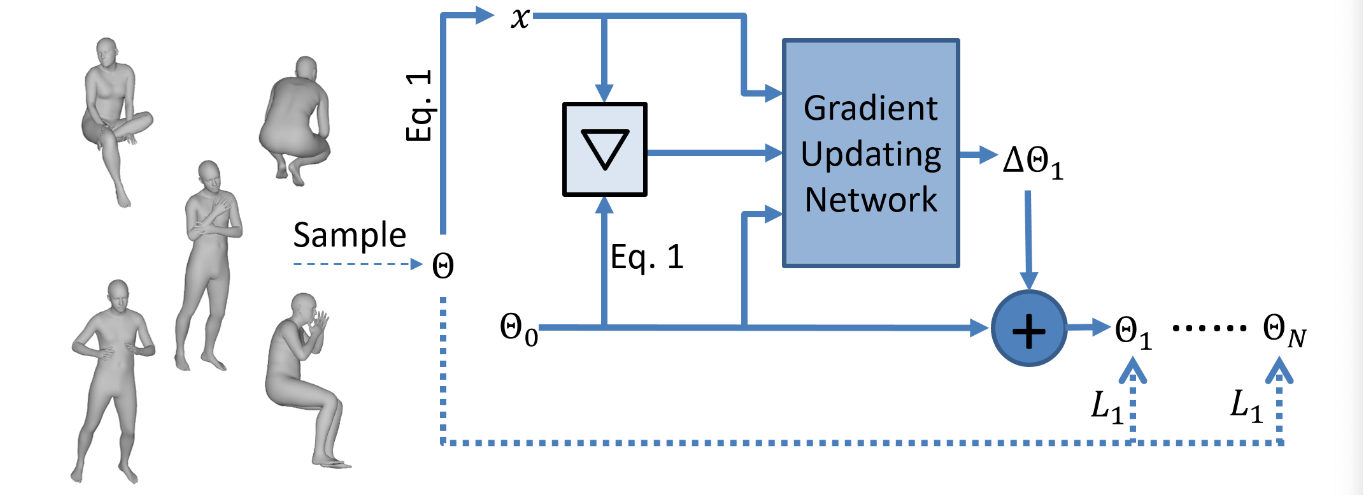
\includegraphics[width=\linewidth]{graphic/pbm-training}
 		\captionof{figure}{PBM Inference Training}
	\end{Figure}
\end{comment}

\textbf{Points to Surfaces}\\
\begin{comment}
	Challenges:
	\begin{itemize}
	\item Self-occlusion
	\item Lack of depth information
	\item Articulated motion
	\item Non-rigid deformation	
	\end{itemize}
\end{comment}